\documentclass[a4paper,10pt]{article}
\usepackage[margin=1in, paperwidth=8.5in, paperheight=11in]{geometry}
\usepackage{amsfonts}
\usepackage{amssymb}
\usepackage[T1]{fontenc}
\usepackage{fancyvrb}
\usepackage[utf8]{inputenc}
\usepackage[english, italian]{babel}
\usepackage{tabularx}
\inputencoding{utf8}
\usepackage{fancyhdr}
\usepackage{graphicx}
\pagestyle{fancy}
\renewcommand{\topfraction}{.9}
\renewcommand{\bottomfraction}{.9}
\renewcommand{\textfraction}{.1}
\fancyhf{}
\lfoot{Qontainer - Elisabetta Piombin - 1142189}


\begin{document}
\title {Relazione del progetto di Programmazione ad Oggetti: Qontainer}
\author {Elisabetta Piombin 1142189}
\date{}

\maketitle
\clearpage
\tableofcontents
\clearpage\mbox{}

\section{Abstract}
\textbf{Qontainer} è un progetto realizzzato al fine di fornire un contenitore che gestisca una libreria di contenuti multimediali: file audio e file video, che si dividono a loro volta in canzoni, podcast, serie tv e film. \\
Per farlo, la classe templatizzata \texttt{container} a sua volta fa uso di altre classi annidate:
\begin{enumerate}
\item \texttt{nodo}: inserita nella parte privata di \texttt{container}, viene usata per memorizzare i vari contenuti multimediali, visti come se fossero una lista concatenata di elementi, con ogni nodo diviso nel suo campo \texttt{info} (di tipo parametrico \texttt{T} e \texttt{next} (di tipo \texttt{nodo*}). In \texttt{container} è presente un puntatore al primo elemento della lista.
\item \texttt{const\_iterator}: inserita nella parte pubblica di \texttt{container}, è la classe che permette l'implementazione di iteratori costanti.
\item \texttt{iterator}: inserita nella parte pubblica di \texttt{container}, è la classe che permette l'implementazione di iteratori non costanti.
\end{enumerate}
Vista l'assenza di puntatori ad altre classi nella gerarchia, è stata ritenuta superflua l'implementazione di una classe per un eventuale \textit{smart pointer}.\\
Ho scelto di implementare il contenitore come una lista linkata composta da nodi perché offro la possibilità di rimuovere contenuti all'interno della libreria in posizioni arbitrarie, e questo mi porta alla necessità di scegliere l'implementazione sotto forma di lista, che rende tale operazione di rimozione più efficiente (viene operata in tempo costante) rispetto alla scelta di implementare tale contenitore come un vettore di elementi.

\section{Compilazione ed esecuzione} 

\section{Descrizione della gerarchia di classi}
La classe base astratta da cui deriva tutta la gerarchia è \texttt{ContenutoMultimediale}, che verrà poi concretizzata tramite sue classi derivate. I metodi virtuali sono \texttt{riproduci()}, \texttt{pausa()}, \texttt{operator==} e il relativo distruttore; \texttt{riproduci()} e \texttt{pausa()} sono anche puri, poiché la loro implementazione è assegnata alle classi derivate. \\
Da \texttt{ContenutoMultimediale} derivano immediatamente altre due classi: \texttt{audio} e \texttt{video}, che sono le due macrocategorie di appartenenza dei file che vengono memorizzati nella libreria. \\
Da \texttt{video} derivano due classi: \texttt{film} e \texttt{episodio}, mentre da \texttt{audio} derivano altre due classi, \texttt{podcast} e \texttt{canzone}. \\
Non si verifica la situazione di ereditarità multipla. \\
\begin{figure}[!htb]
	\center{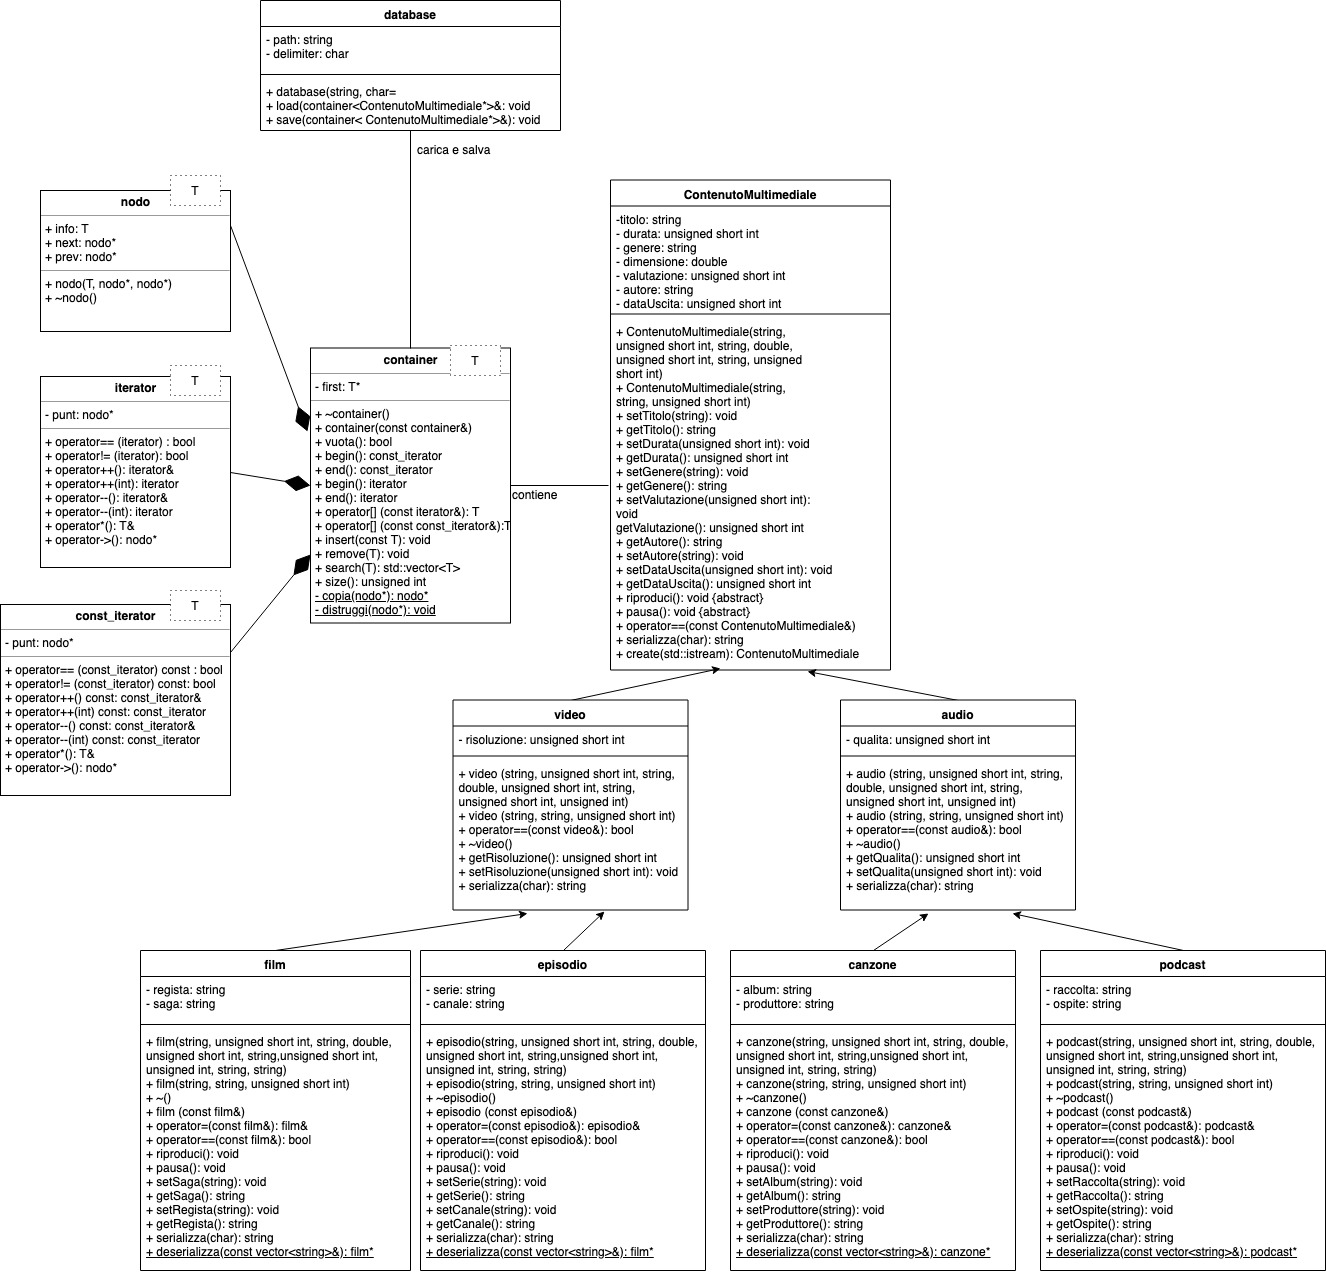
\includegraphics[width=\textwidth]
		{uml.jpg}}
	\caption{\label{fig:my-label} Diagramma delle classi del modello}
\end{figure}

\section{Descrizione delle chiamate polimorfe}
Le chiamate polimorfe vengono pesantemente utilizzate nelle operazioni di modifica, rimozione, ricerca e aggiunta degli elementi nel contenitore, in quanto il contenitore viene istanziato a \texttt{<ContenutoMultimediale*>}, e tramite \textit{downcasting} (via \texttt{dynamic\_cast}) effettuato al Tipo desiderato, si eseguono le operazioni necessarie sui tipi.\\
Le chiamate polimorfe presenti nel progetto sono le seguenti:
\begin{enumerate}
\item[-] nella \textit{mainwindow} dell'applicazione, dove vengono elencati tutti i contenuti presenti nel contenitore: questa operazione è eseguita tramite downcasting da \texttt{ContenutoMultimediale*} al tipo target desiderato alla base della gerarchia.
\item[-] nelle finestre di aggiunta dei contenuti e di ricerca, all'interno della funzione \texttt{aggiungiInput()}, necessaria per caricare i box di testo e le rispettive etichette necessarie per il tipo di contenuto multimediale selezionato precedentemente nel menù a tendina.
\item[-] dentro al file \texttt{qontainer.cpp}, necessario per il corretto caricamento di tutte le finestre e dell'eliminazione della finestra corrente per far caricare correttamente la finestra successiva: nella funzione \texttt{eliminaContenutoAttuale()} viene usato un \texttt{dynamic\_cast} necessario per la corretta eliminazione del \textit{layout} attuale, effettuando un \textit{downcast} a \texttt{QWidgetItem}.
\item[-] dentro al file \texttt{risultatoricerca.cpp} viene usato il \textit{downcasting} per visualizzare a schermo il tipo dinamico dei puntatori ad oggetti contenuti nel contenitore che è stato ritornato come risultato dalla funzione \texttt{search(ContenutoMultimediale*)}.
\item[-] nell'aggiunta di contenuto nel contenitore tramite GUI, attraverso la funzione \texttt{aggiungiElemento()} all'interno del file \texttt{aggiungi.cpp}, l'aggiunta viene eseguita tramite un puntatore di tipo statico \texttt{Contenuto Multimediale*}, ma tipo dinamico differente a seconda del tipo di file che si vuole aggiungere nel contenitore.
\end{enumerate}



\section{Descrizione del formato del file di salvataggio e caricamento del contenitore}
Per il caricamento dei file che compongono la libreria, e per il loro salvataggio, mi appoggio ad una classe esterna alla gerarchia, che ho chiamato \texttt{database}. Questa classe contiene i metodi \texttt{load()} e \texttt{save()}: 
\begin{enumerate}
\item[-] \texttt{load()}, tramite un'operazione di deserializzazione implementata ad hoc in ogni classe derivata concreta della gerarchia, permette la lettura del contenuto in ogni file \texttt{.txt}. C'è un file \texttt{.txt} per ognuna delle classi \texttt{film}, \texttt{episodio}, \texttt{canzone} e \texttt{podcast}, con relativa funzione di deserializzazione, che trasforma ogni riga contenuta in quei file in oggetto della relativa classe. Database si occupa di caricare questi oggetti nella libreria, in modo che possano essere gestiti dal contenitore templetizzato.
\item[-] \texttt{save()} invece si occupa del salvataggio di eventuali modifiche apportate tramite GUI ai file \texttt{.txt} sovramenzionati, tramite le relative operazioni di serializzazione, contenute nelle relative classi. 
\end{enumerate}

\section{Tempistiche}

\begin{center}
 \begin{tabular}{||c | c ||} 
 \hline
 \textbf{Ore} & \textbf{Fase}  \\ 
 \hline\hline
 2 & Analisi preliminare del problema \\ 
 \hline
 1 & Progettazione del modello \\
 \hline
 1 & Progettazione della GUI\\
 \hline
 10 & Apprendimento libreria Qt \\
 \hline
 30 & Codifica modello e GUI\\ 
 \hline
 10 & Debugging \\
 \hline
 5 & Testing\\
 \hline
\end{tabular}
\end{center}

\end{document}